\documentclass[10pt]{beamer}

\usetheme[progressbar=frametitle]{metropolis}
\usepackage{appendixnumberbeamer}

\usepackage{booktabs}
\usepackage[scale=2]{ccicons}

\usepackage{pgfplots}
\usepgfplotslibrary{dateplot}
\usepackage[portuguese]{babel}
\usepackage{amsmath}
\usepackage{bm}
\usepackage{cleveref}

\usepackage{minted}

\usepackage{xspace}
\newcommand{\themename}{\textbf{\textsc{metropolis}}\xspace}

\title{
\includegraphics[scale=0.15]{figuras/logo-ipt.pdf} \hfill 
\includegraphics[scale=0.1]{figuras/usp-logo.pdf}\\Exame de qualificação de mestrado}
\subtitle{Aprendizagem de representação através do uso de redes neurais convolucionais na recuperação de trecho de código-fonte}
% \date{\today}
\date{}
\author{Marcelo de Rezende Martins\\{\footnotesize sob orientação do Prof. Dr. Marco Aurélio Gerosa}}
\institute{Instituto de Pesquisas Tecnológicas do Estado de São Paulo - IPT}
% \titlegraphic{\hfill\includegraphics[height=1.5cm]{logo.pdf}}

\begin{document}

\maketitle



\section[Intro]{Introdução}


\begin{frame}[fragile]{Definição}

\begin{quote}
Recuperação de trecho de código-fonte consiste em recuperar um trecho de código a partir de um repositório de códigos-fontes, de modo a atender a intenção do desenvolvedor, expressa em linguagem natural \footnote{Jose Cambronero, Hongyu Li, Seohyun Kim, Koushik Sen, and Satish Chandra. 2019. When deep learning met code search.}\footnote{Xiaodong Gu, Hongyu Zhang, and Sunghun Kim. 2018. Deep code search.}.     
\end{quote}


\end{frame}
\begin{frame}[fragile]{Definição (ERRATA)}

  \textbf{Code Retrieval}: Dada uma questão em linguagem natural $q \in \mathbb{Q}$, um modelo $F_{r}$ será treinado a recuperar os trechos $\mathbb{C}^{+} \subset \mathbb{C}_{a}$ com a maior pontuação:

\begin{equation}\label{eq:code-retrieval}
\mathbb{C}^{+} = \underset{c \in \mathbb{C}_{a}}{argmax}\text{ } F_{r}(q , c)
\end{equation}
\end{frame}


\section{Abordagem}

\begin{frame}{Joint Embedding}
    Sejam $\mathbb{Q}$ e $\mathbb{C}$ conjuntos de dados heterogêneos. \textit{Joint embedding} pode ser formulado como:
	\begin{equation}
        f: q \rightarrow t_{q} \rightarrow h_{\theta}(t_{q}, t_{c}) \leftarrow t_{c} \leftarrow c :g
    \end{equation}
\end{frame}

\begin{frame}{Joint Embedding}
   \begin{center}
       \begin{tabular}{|p{4cm}|p{4cm}|}
            \hline
            Como representar as palavras e os tokens das questões e trechos de código-fonte? & \textit{Word2Vec} \\ 
            \hline
            Como representar as sentenças? &  CNN \\
            \hline
            Como aproximá-los? &  Função de custo \textit{hinge} \\
            \hline
       \end{tabular}
   \end{center}
\end{frame}

\begin{frame}{Arquitetura}
	\begin{figure}[h]
        \centering
        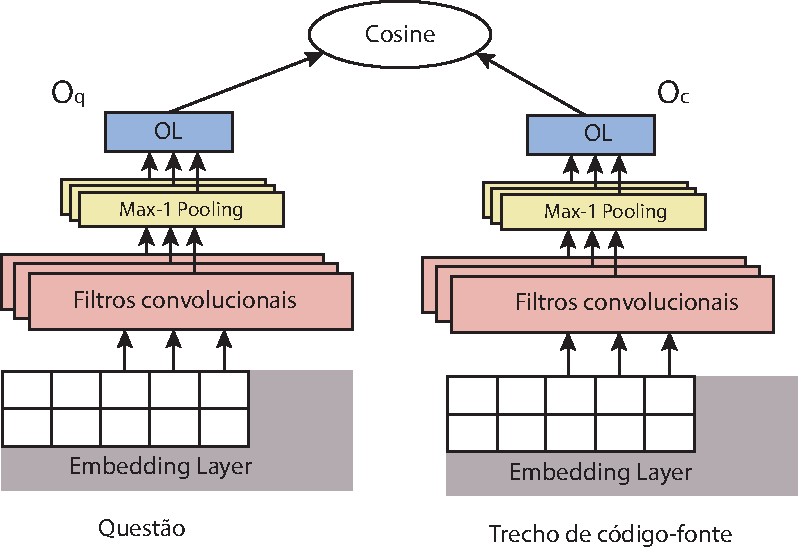
\includegraphics[width=0.8\linewidth]{figuras/cnn-architecture-proposal.pdf}
        \caption{Arquitetura CNN proposta para recuperação de trecho de código-fonte.}
        \label{fig:cnn-architecture-proposal}
    \end{figure}
\end{frame}


\begin{frame}{CNN}
	\begin{figure}[h]
        \centering
        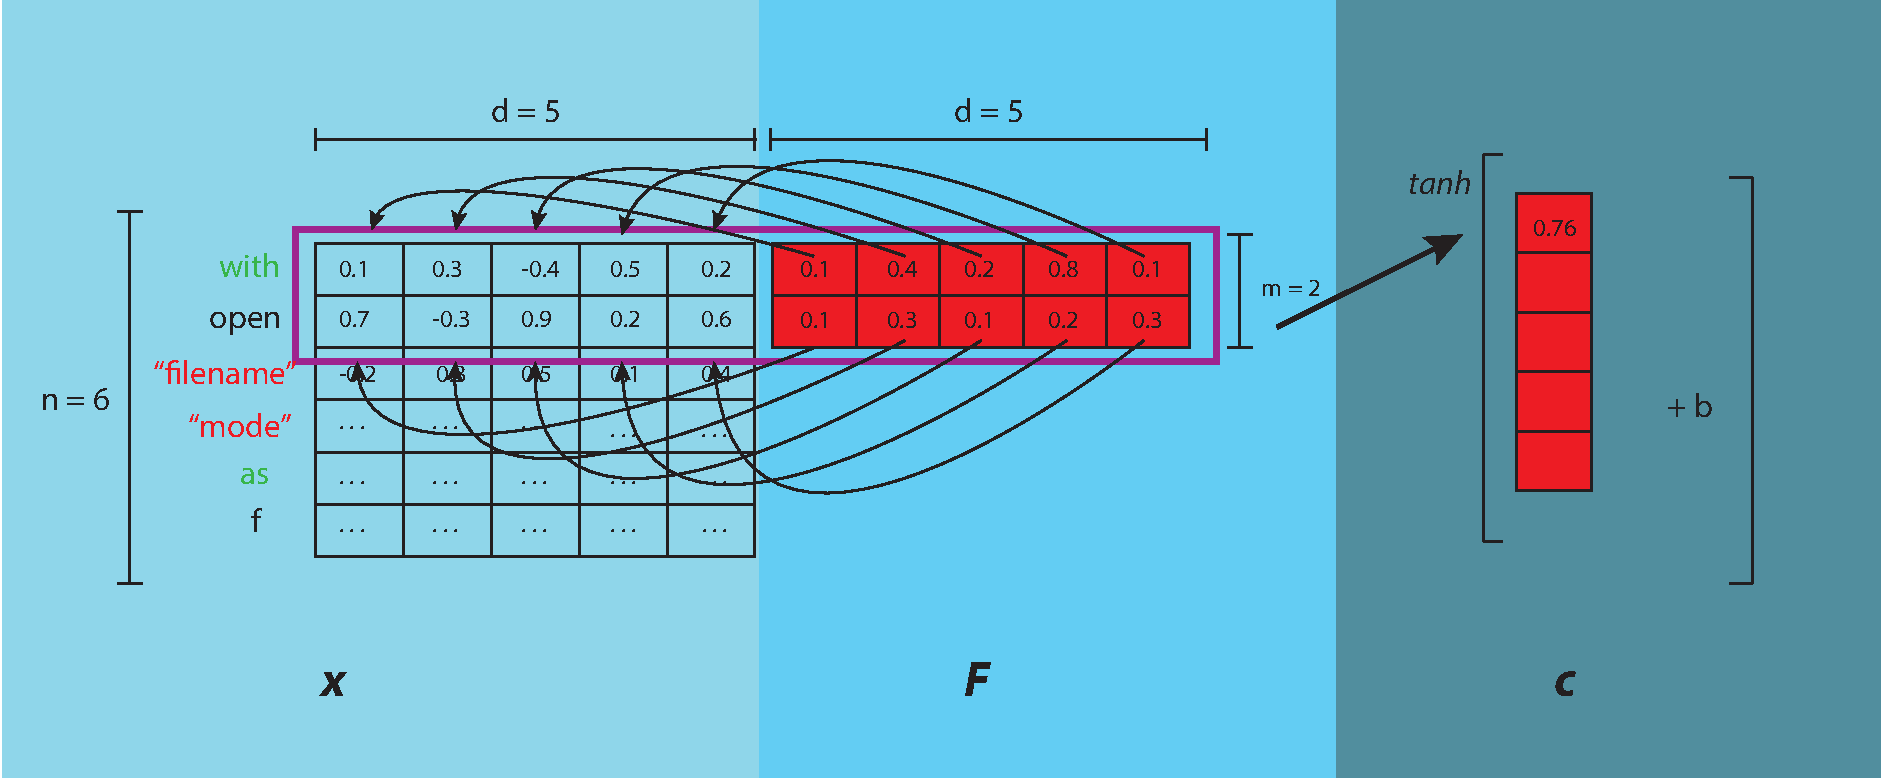
\includegraphics[width=1\linewidth]{figuras/first-step-convolution.pdf}
        \caption{Primeiro passo da operação de convolução em um vetor de entrada $\bm{x}$ composto por vetores de representação distribuída de cada palavra da sentença. }
        \label{fig:first-step-convolution}
    \end{figure}
\end{frame}

\section{Questões}


\begin{frame}{Questões}
	\begin{itemize}
	    \item A aprendizagem de representação através do CNN auxilia na recuperação de trecho de código-fonte?
	    \item O CNN é capaz de extrair as características mais relevantes de modo a facilitar o modelo a encontrar uma correlação entre as questões e os trechos de código-fonte?
	\end{itemize}
	Indiretamente:
	\begin{itemize}
	    \item As interações locais auxiliam na aproximação das intenções aos trechos de código?
	\end{itemize}
\end{frame}

\begin{frame}{Avaliação}
   \begin{center}
       \begin{tabular}{|p{4cm}|p{4cm}|}
            \hline
            Dados de treinamento & Conjunto de pares de questões e trechos de código-fonte em Python coletados do Stack Overflow por Yao et al. (2018)\footnote{\label{foot:yao-staqc}Yao, Ziyu and Weld, Daniel S. and Chen, Wei-Peng and Sun, Huan. 2018. StaQC: A Systematically Mined Question-Code Dataset from Stack Overflow} \\ 
            \hline
            Dados para avaliação final & Conjunto de dados anotados manualmente e disponibilizados por Yao et al. (2018)\textsuperscript{\ref{foot:yao-staqc}} \\
            \hline
            Métrica de desempenho & \emph{MRR} \\
            
            
            \hline
       \end{tabular}
   \end{center}
\end{frame}

\begin{frame}{Avaliação}
   \begin{center}
       \begin{tabular}{|p{4cm}|p{4cm}|}
       \hline
            Arquiteturas de referência para comparação & \begin{itemize}
                \item Embedding
                \item Rede neural com mecanismo de atenção proposto por Cambronero et al. (2019)\footnote{Jose Cambronero, Hongyu Li, Seohyun Kim, Koushik Sen, and Satish Chandra. 2019. When deep learning met code search.}
            \end{itemize} \\
            
            \hline
       \end{tabular}
   \end{center}
\end{frame}

\begin{frame}{Avaliação}
   \begin{center}
       \begin{tabular}{|p{4cm}|p{4cm}|}
       
            \hline
            Análise dos resultados & \begin{itemize}
                \item Inspeção manual
                \item Análise dos piores casos
                \item Patologia das redes neurais (Feng et al. , 2018)\footnote{Shi Feng, Eric Wallace, Alvin Grissom II, Mohit Iyyer, Pedro Rodriguez, Jordan Boyd-Graber. 2018. Pathologies of Neural Models Make Interpretations Difficult.}
            \end{itemize} \\
            \hline
       \end{tabular}
   \end{center}
\end{frame}

\section{Experimento piloto}


\begin{frame}{Resultados preliminares\footnote{Marcelo de Rezende Martins e Marco Aurélio Gerosa. 2019. Um estudo preliminar sobre o uso de uma arquitetura deep learning para seleção de respostas no problema de recuperação de trecho de código-fonte.}}
  \begin{table}[h]
\centering
\begin{tabular}{ p{3cm} p{3cm} }
 \hline
 \textbf{Modelos} & \textbf{Resultados (MRR)}\\
 \hline
 Embedding & $0,52 \pm 0,01$\\
 
 \textcolor{blue}{\textbf{CNN}} & \textcolor{blue}{$\bm{0,58} \pm \bm{0,01}$} \\
 
 \textbf{bi-LSTM-CNN} & $\bm{0,60} \pm \bm{0,02}$\\
 \hline
\end{tabular}
\caption[Resultado preliminar]{Resultado preliminar do modelo CNN em comparação com outras duas arquiteturas (bi-LSTM com CNN e Embedding). Estes resultados foram obtidos a partir da amostra EVAL.}
\end{table}
\end{frame}

\begin{frame}{Histograma das posições dos trechos de código-fonte relevantes}
  \begin{figure}[h]
    \centering
    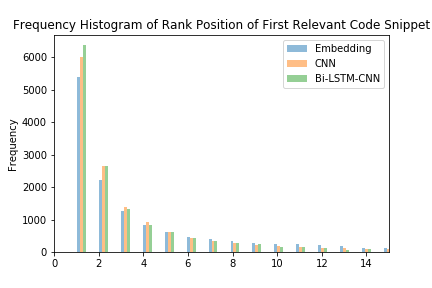
\includegraphics[width=1\textwidth]{figuras/histogram_results.png}
    \label{fig:histogram-results}
\end{figure}
\end{frame}

\begin{frame}[fragile]{Exemplos}
        \alert{Python and appending items to text and \colorbox{green}{excel} \colorbox{green}{file}}\footnote{{\tiny \url{https://stackoverflow.com/questions/24593478/python-and-appending-items-to-text-and-excel-file}}}
        \metroset{block=fill}
        \begin{exampleblock}{BiLSTM-CNN}
        \begin{minted}[breaklines,fontsize=\scriptsize, escapeinside=||]{python}
Yvalues = [1, 2, 3, 4, 5]
file_out = |\colorbox{green}{open}|('file.csv','wb')
mywriter=|\colorbox{green}{csv}|.|\colorbox{green}{writer}|(file_out, delimiter = '\n')
mywriter.|\colorbox{green}{writerow}|(Yvalues)
file_out.close()
        \end{minted}
        \end{exampleblock}
        \begin{alertblock}{CNN}
        \begin{minted}[breaklines,fontsize=\scriptsize, escapeinside=||]{python}
import csv

with |\colorbox{green}{open}|("output.csv", "wb") as f:
    writer = |\colorbox{green}{cwv}|.|\colorbox{green}{writer}|(f)
    writer.|\colorbox{green}{writerows}|(a)
    \end{minted}
    \end{alertblock}
    
\end{frame}

\section{Próximos passos}

\begin{frame}{Próximas tarefas}
    \begin{itemize}
        \item Implementação da arquitetura proposta por Cambronero et al. (2019)\footnote{Jose Cambronero, Hongyu Li, Seohyun Kim, Koushik Sen, and Satish Chandra. 2019. When deep learning met code search.}
        \item Adição de regularização aos modelos
        \item Coleta e análise dos resultados
    \end{itemize}
\end{frame}


{\setbeamercolor{palette primary}{fg=black, bg=yellow}
\begin{frame}[standout]
  Perguntas?
\end{frame}
}

\appendix





\end{document}
